\subsection{Overview}



%---------------------------------------------------------


\subsection{KUKA Robot Arm}

\subsubsection{Suggested Reading}

\subsubsection{Introduction}









%---------------------------------------------------------


\subsection{3-Axis Linear Stage}


\subsubsection{Suggested Reading}

\paragraph{Datasheets}

\begin{itemize}

    \item \href{link}{title}
    
    \item \href{link}{title}

\end{itemize} 



\subsubsection{Introduction}

\subsubsection{Parts List}

\subsubsection{Assembly}
\paragraph{Linear X-Stage}

\begin{enumerate}

\item Place the long Guide Rail in the X-stage Rail base and loosely attach it with M4 16mm screws as shown in figure \ref{fig:xaxis3}



\item Screw the base plate to the Ball Bearing Carriage using M3 8mm screws, then screw the base plate to the X-axis Ball Nut Bracket with M3 10mm screws. 

\begin{figure}
\centering
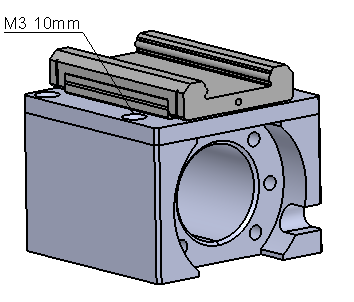
\includegraphics[scale=0.5]{Platforms/figs/xaxis2.png}
\caption{\label{fig:xaxis2}}
\end{figure}

\item At one end of the Base rail attach the floating end brackets using M5 22mm screws. If the tolerance is not sufficiently tight, washers can be used as a buffer between the components.

\begin{figure}
    \centering
    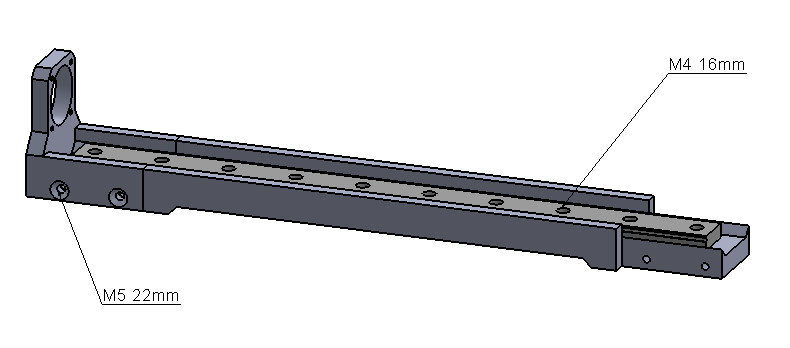
\includegraphics[scale=0.5]{Platforms/figs/xaxis3.png}
    \caption{\label{fig:xaxis3}}
\end{figure}

\item Attach the floating bearing block to the floating end bracket using M4 12mm screws.

\item Insert a ball screw in the ball nut bracket and secure with M5 12mm screws.

\item Attach the fixed bearing block on the side of the ball screw containing smaller threads. The fixed bearing block should be inserted such that the threads are exposed on the open end of the ball screw.

\item Attach the motor coupling to the same end of the ball screw.

\begin{figure}
    \centering
    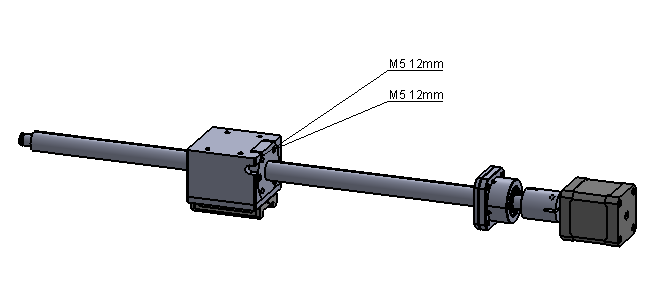
\includegraphics[scale=0.5]{Platforms/figs/xaxis4.png}
    \caption{\label{fig:xaxis4}}
\end{figure}

\item Slide the ball bearing carriage along with the rest of the attached ball screw onto the the attached base rail. push the end without a motor couple through the floating bearing block. The result should look like figure \ref{fig:xaxis5} 

\begin{figure}
    \centering
    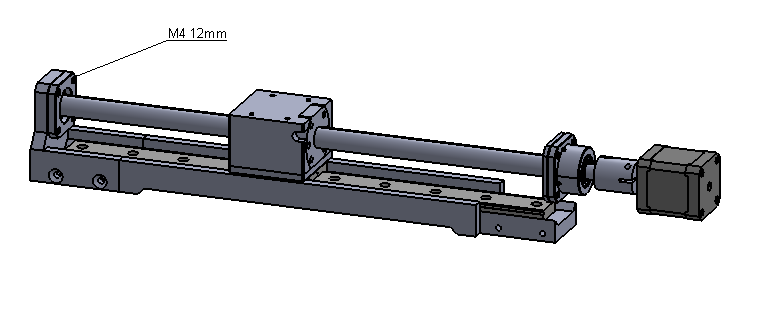
\includegraphics[scale=0.4]{Platforms/figs/xaxis5.png}
    \caption{\label{fig:xaxis5}}
\end{figure}

\item Insert the fixed end brackets and secure them with the rail base using M4 16mm screws.If the tolerance is not sufficiently tight, washers can be used as a buffer between the components. 

\item Attach the fixed bearing block with the fixed end ball nut bracket using the M4 12mm screws. 

\item Attach the motor to the open end of the fixed end bracket using M3 12mm screws. 

\item Tighten the screws attaching the guide rail and the rail base once everything is aligned and secure.It should look like figure \ref{fig:xaxis6}

\begin{figure}
    \centering
    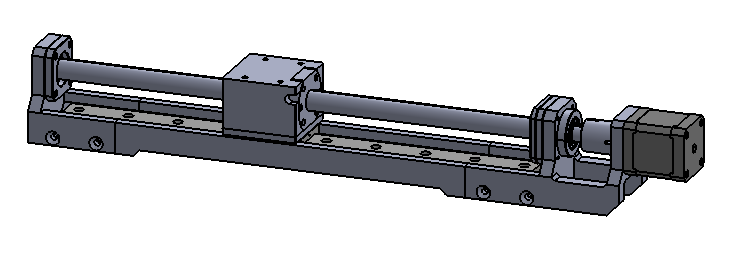
\includegraphics[scale=0.4]{Platforms/figs/xaxis6.png}
    \caption{\label{fig:xaxis6}}
\end{figure}

\end{enumerate}




\paragraph{Y-axis Linear stage}

\begin{enumerate}

\item Align the floating end bracket and the z-axis ball nut bracket. Attach the two pieces using M5 22mm and M5 13mm screw as shown in figure \ref{fig:yaxis3}


\begin{figure}
    \centering
    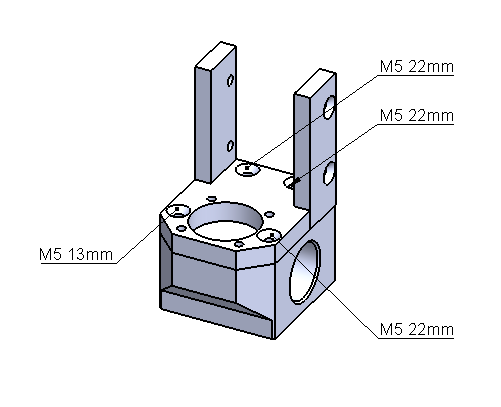
\includegraphics[scale=0.6]{Platforms/figs/yaxis3.png}
    \caption{\label{fig:yaxis3}}
\end{figure}

\item Place the floating bearing block in the floating end bracket and secure it with M4 23.5mm screws at the top as indicated in figure \ref{fig:yaxis4}

\begin{figure}
    \centering
    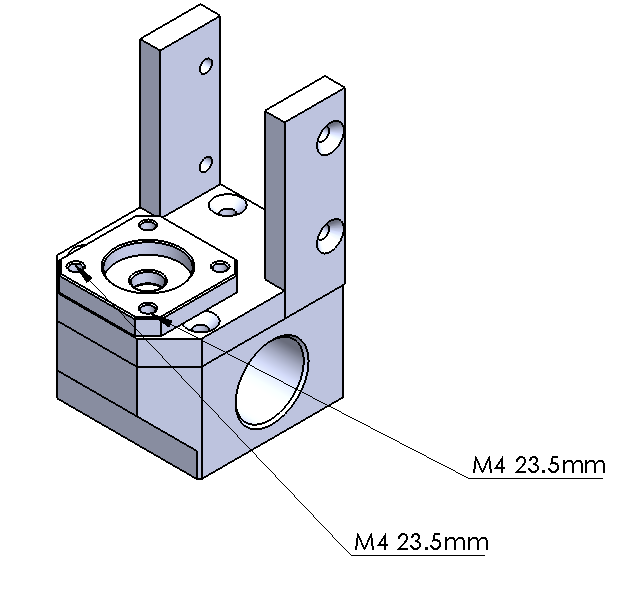
\includegraphics[scale=0.4]{Platforms/figs/yaxis4.png}
    \caption{\label{fig:yaxis4}}
\end{figure}

\item Attach the floating end bracket to the rail base with M5 22mm screws and position the guide rail on top of the rail base. Join the rail base and guide rail loosely using M4 16mm screws as shown in figure \ref{fig:yaxis5}.

\begin{figure}
    \centering
    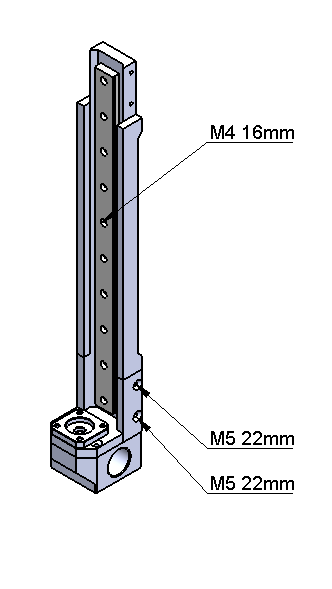
\includegraphics[scale=0.5]{Platforms/figs/yaxis5.png}
    \caption{\label{fig:yaxis5}}
\end{figure}

\item Attach the rail carriage adaptor with the ball bearing carriage using M3 8mm screws. Then screw the rail carriage adaptor to the ball nut bracket as shown in the figure \ref{fig:yaxis6} using the M3 10mm screws.

\begin{figure}
    \centering
    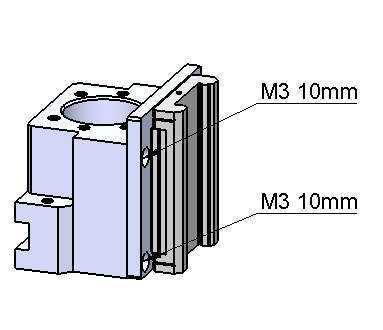
\includegraphics[scale=0.6]{Platforms/figs/yaxis6.png}
    \caption{\label{fig:yaxis6}}
\end{figure}

\item Insert the ball nut screw into the Y-axis ball nut bracket, and secure the pieces using M5 22mm screws, then slide the carriage and the ball nut screw on top of the rail. figure \ref{fig:yaxis7} (THE BRACKET FPR THE SENSORS HAVE NOT BEEN ADDED)
    
\begin{figure}
    \centering
    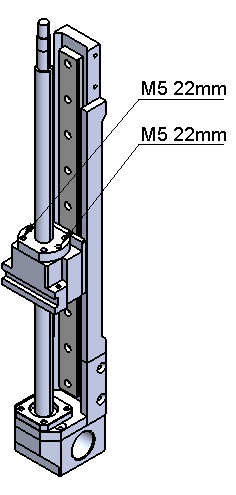
\includegraphics[scale=0.6]{Platforms/figs/yaxis7.png}
    \caption{\label{fig:yaxis7}}
\end{figure}

\item Repeat steps 4-12 from the X-axis linear system instructions with the corresponding Y-axis components. The Y-axis linear system should then look like the figure \ref{fig:yaxis8}

\begin{figure}
    \centering
    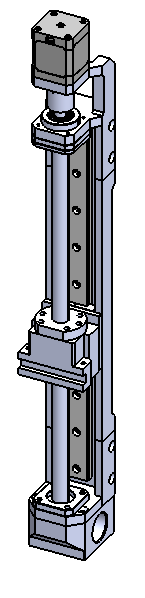
\includegraphics[scale=0.6]{Platforms/figs/yaxis8.png}
    \caption{\label{fig:yaxis8}}
\end{figure}
 
\end{enumerate}


\paragraph{Z-axis linear stage}
\begin{enumerate}

\item Attach the Z-axis Rail base to the A-axis ball nut bracket using M5 22mm (CHECK FROM HERE) screws as shown in figure \ref{fig:zaxis1}.

\begin{figure}
    \centering
    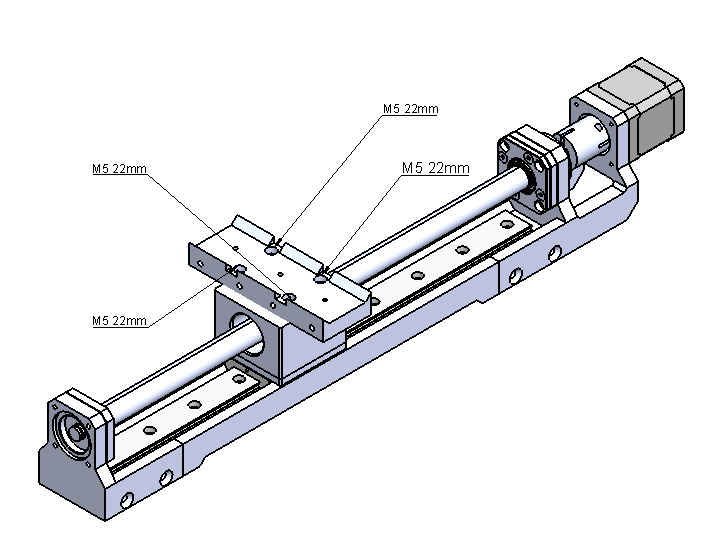
\includegraphics[scale=0.5]{Platforms/figs/zaxis1.png}
    \caption{\label{fig:zaxis1}}
\end{figure}

\item Loosely secure the small Guide rail on the base rail using M4 16mm screws, Attach the floating end bracket with the base Rail using M5 22mm screws.

\item To the floating end bracket attach the 

\item Attach the rail carriage adaptor with the ball bearing carriage using M3 8mm screws. Then screw the rail carriage adaptor to the ball nut bracket at the end of Y-axis linear stage as shown in the figure  using the M3 10mm screws.

\item Slide the carriage on the rail and push the ball nut screw threw ball nut bracket and secure it with the bracket using????? screws (NEED INFORMATION)


\end{enumerate}

\subsubsection{Maintenance}